\documentclass[landscape]{slides}
\usepackage[landscape, margin=2cm]{geometry}
\usepackage{color}
\usepackage{bm}
\usepackage{graphicx}
\usepackage{hyperref}
\graphicspath{ {./img/} {./charts/} }



\title{Show and Tell: Skill Acquisition}
\author{Adam Johnson - me@adamj.eu}
\date{28th August 2013}

\begin{document}

\maketitle


\begin{slide}

    \textcolor{blue}{\Large{I have been learning a skill...}}

\end{slide}


\begin{slide}

    \textcolor{blue}{\Large{...what is it?}}

    \begin{itemize}
        \item Something you did today
        \item You've been paid to do it
        \item You've probably never \emph{really} practiced it in your life...
    \end{itemize}


    % no, it's not making tea...

\end{slide}


\begin{slide}

    \textcolor{blue}{\Large{Typing!}}

    \centering

    
\includegraphics[height=10cm]{baby-nerd}

    (not me)

\end{slide}


\begin{slide}

    \textcolor{blue}{\Large{Motivation}}

    \begin{itemize}
        \item I'm a programmer - I have \emph{a lot} of typing to do!
        \item Fear of RSI - colleagues have been crippled by it
        % \item Always \emph{intended} to learn to touchtyping
        \item Statistic: ``In the USA, carpal tunnel syndrome results in an average of \$30,000 in lifetime costs'' \small{(Wikipedia)}
    \end{itemize}

\end{slide}


\begin{slide}

    \textcolor{blue}{\Large{To business!}}

    \begin{itemize}
        \item Just need to grab some typing programs
        \item Get down to learning QWERTY the \emph{right} way!!
    \end{itemize}

\end{slide}


\begin{slide}

    \textcolor{blue}{\Large{Ten Thumbs}}

    \centering

    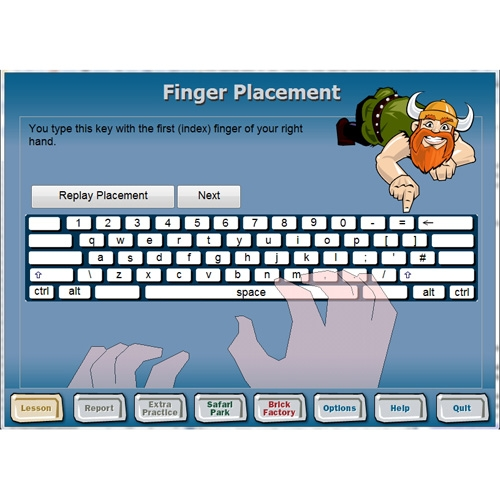
\includegraphics[height=15.5cm]{ten-thumbs}

\end{slide}


\begin{slide}

    \textcolor{blue}{\Large{Oh no....}}

\end{slide}

\begin{slide}
    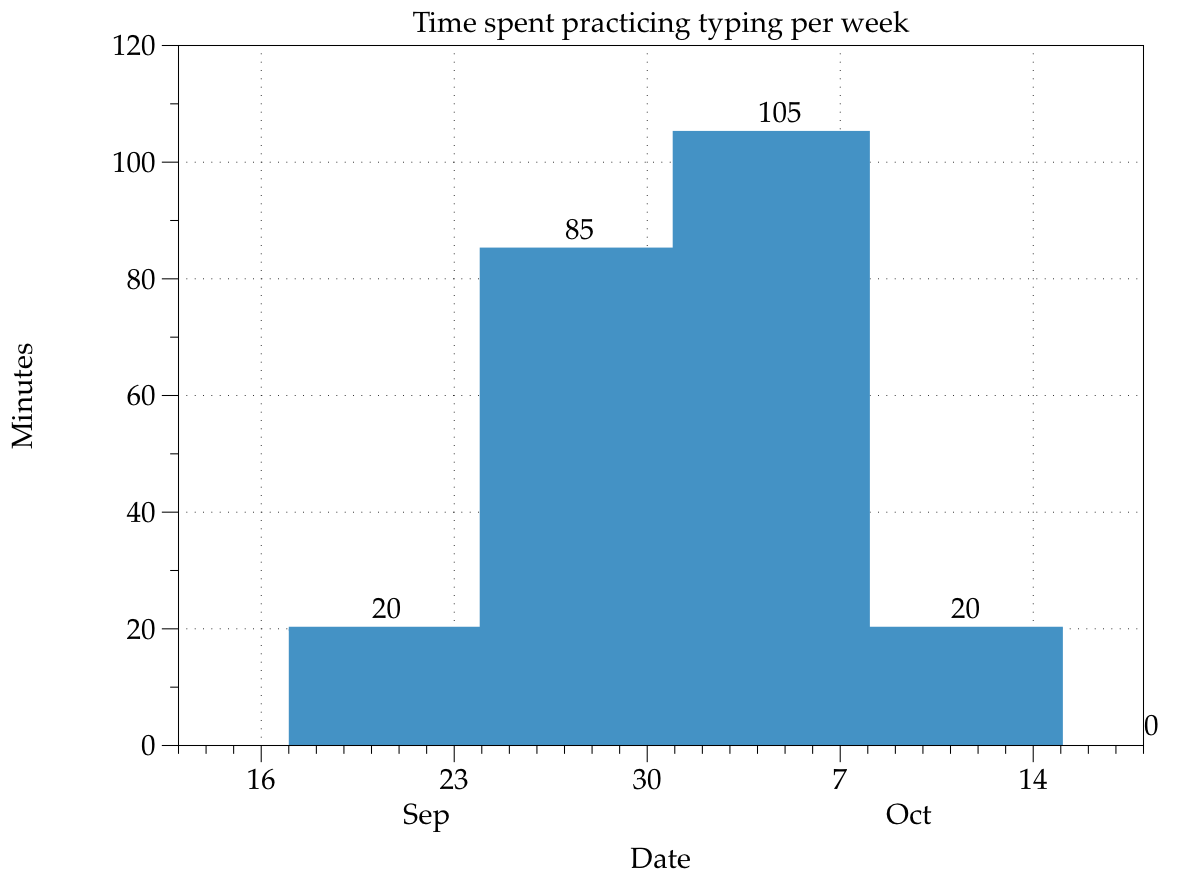
\includegraphics[width=\textwidth]{first-practice}
\end{slide}

\begin{slide}
    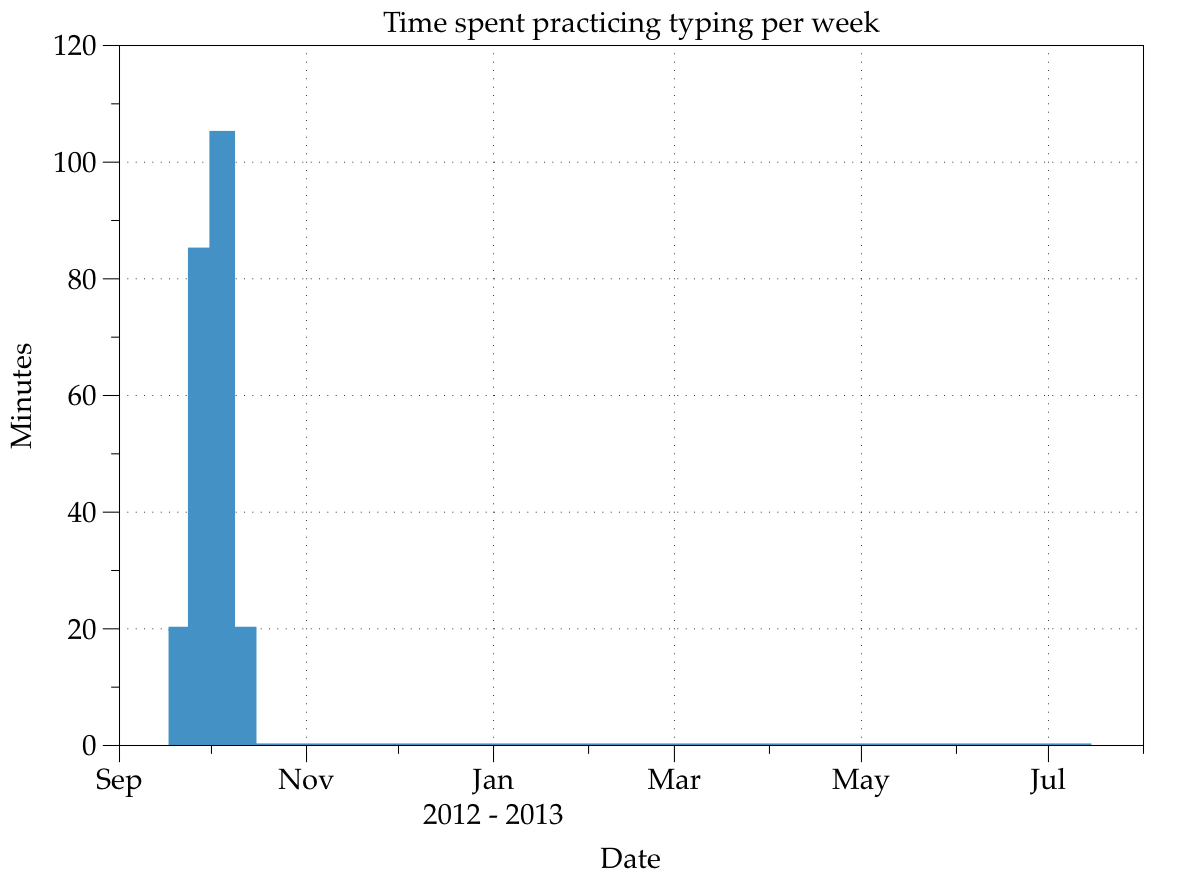
\includegraphics[width=\textwidth]{first-practice-long-tail}
\end{slide}


\begin{slide}
    
\includegraphics[width=\textwidth]{homer}
\end{slide}


\begin{slide}

    \textcolor{blue}{\Large{Undefined}}

    \begin{itemize}
        \item Didn't know how long it would take
        \item Is this really the best idea?
        \item Hard practicing QWERTY \emph{the right way} at night, then going back to old habits during the day
    \end{itemize}

\end{slide}


\begin{slide}

    \textcolor{blue}{\Large{...what changed?}}

\end{slide}


\begin{slide}

    \textcolor{blue}{\Large{A Book}}

    \centering

    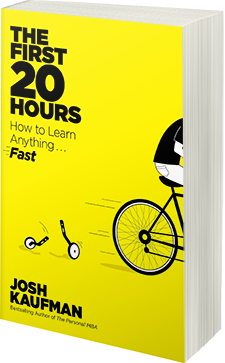
\includegraphics[height=13cm]{first20hours-cover}

    \begin{itemize}
        \item Josh Kaufman, 2013 - \url{http://first20hours.com/}
    \end{itemize}

\end{slide}


\begin{slide}

    \textcolor{blue}{\Large{The First 20 Hours : Rapid Summary}}

    \begin{itemize}
        \item Nearly any skill can be learnt (to a useful degree) in 20 hours
        \item A couple chapters of general how-to, then one chapter on each of six skills he learnt with his method
        \item One of these was on touchtyping... in \textbf{`Colemak'}
    \end{itemize}

\end{slide}


\begin{slide}

    \textcolor{blue}{\Large{A brief history of keyboard design...}}

    \centering

    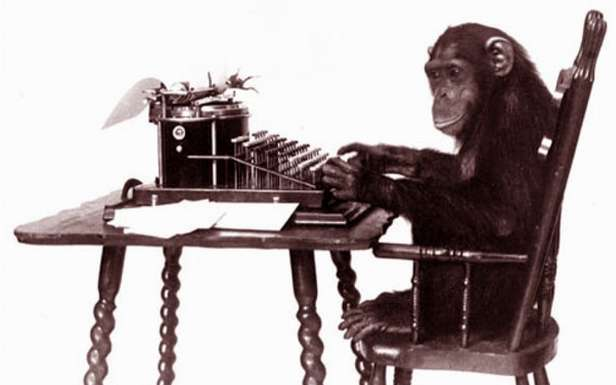
\includegraphics[width=0.9\textwidth]{chimp}

\end{slide}


\begin{slide}

    \textcolor{blue}{\Large{QWERTY}}

    \centering
    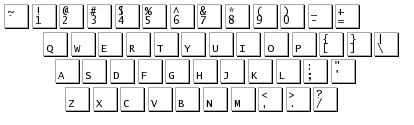
\includegraphics[width=20cm]{qwerty}

    \begin{itemize}
        \item ``Slowly took over the world'', since 1872. Main design constraint: to stop typewriter key bars jamming.
    \end{itemize}

\end{slide}


\begin{slide}

    \textcolor{blue}{\Large{DVORAK}}

    \centering
    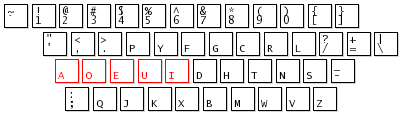
\includegraphics[width=20cm]{dvorak}

    \begin{itemize}
        \item 1932 design for an optimal layout.
        \item Relatively hard to learn.
    \end{itemize}

\end{slide}


\begin{slide}

    \textcolor{blue}{\Large{Colemak}}

    \centering
    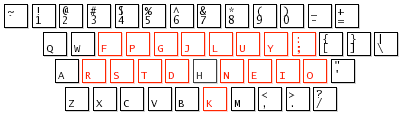
\includegraphics[width=20cm]{colemak-annot}

    \begin{itemize}
        \item Designed by a programmer with a mathematical model and lots of spare time.
        \item Trade-off between ease of transition (Q,W,Z,X,C,V stay the same) and optimization.
    \end{itemize}

\end{slide}


\begin{slide}

    \centering

    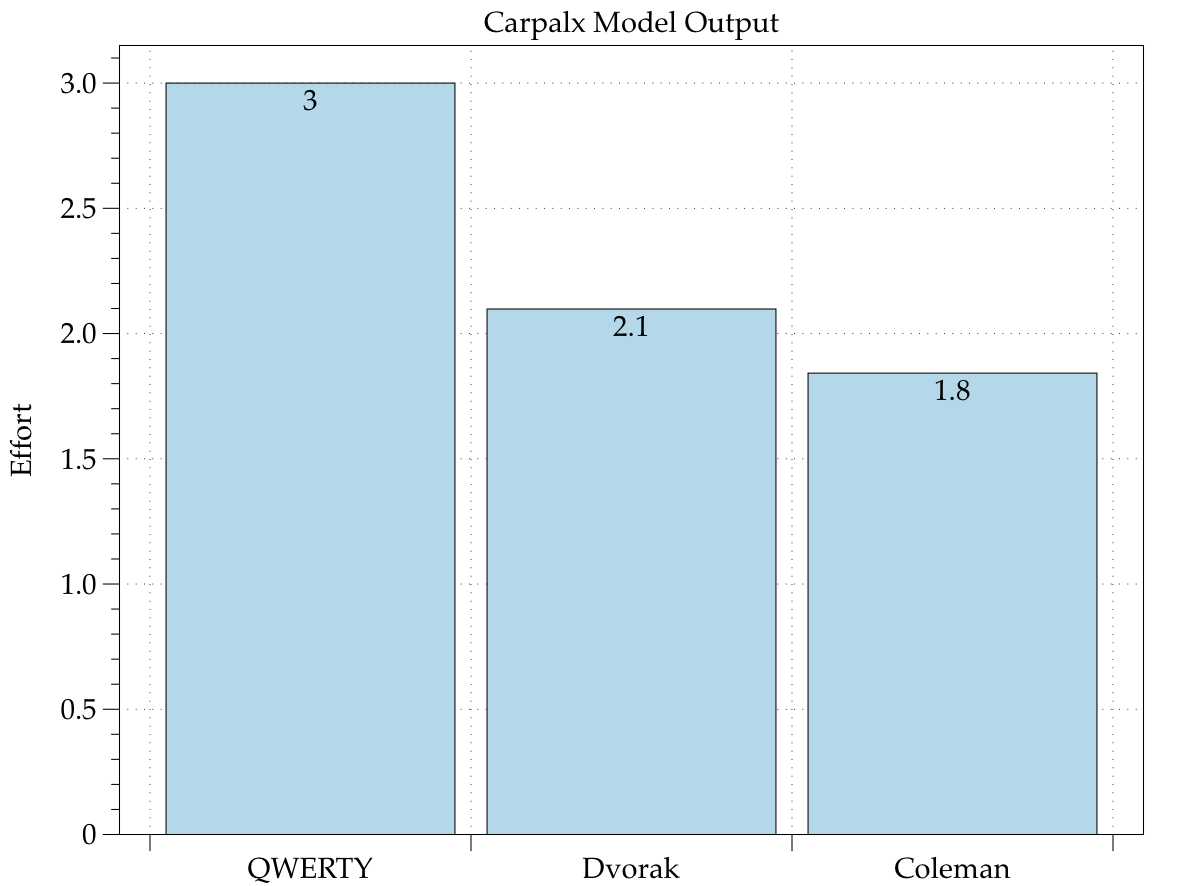
\includegraphics[width=0.85\textwidth]{keyboards}

    \begin{itemize}
        \item Source: \url{http://mkweb.bcgsc.ca/carpalx/?colemak}
    \end{itemize}

\end{slide}


\begin{slide}

    \centering

    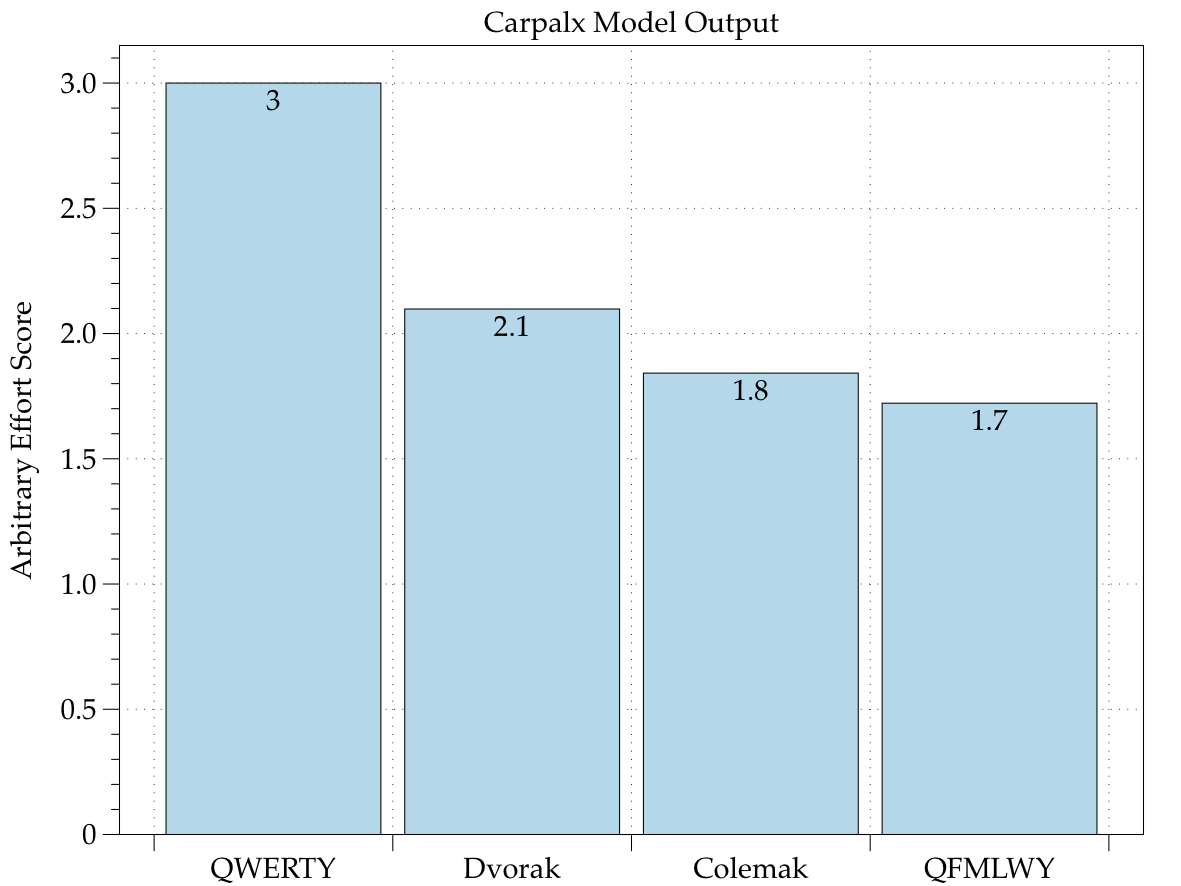
\includegraphics[width=0.85\textwidth]{keyboards-qfmlwy}

    \begin{itemize}
        \item Source: \url{http://mkweb.bcgsc.ca/carpalx/?full_optimization}
    \end{itemize}

\end{slide}


\begin{slide}

    \textcolor{blue}{\Large{Method}}

    \begin{itemize}
        \item Swap keys on OS and keyboard
        \item Get some training programs
        \item Don't give up before the 20 hour mark
    \end{itemize}

\end{slide}


\begin{slide}

    \textcolor{blue}{\Large{Programs}}

    \begin{itemize}
        \item A variety is useful
        \item Practice different subskills - hardest keys, whole prose, etc.
        \item Data export is not much of a feature. Many record your WPM + accuracy, but often only for own graph feature.
    \end{itemize}

\end{slide}


\begin{slide}

    \textcolor{blue}{\Large{Amphetype}}

    \centering

    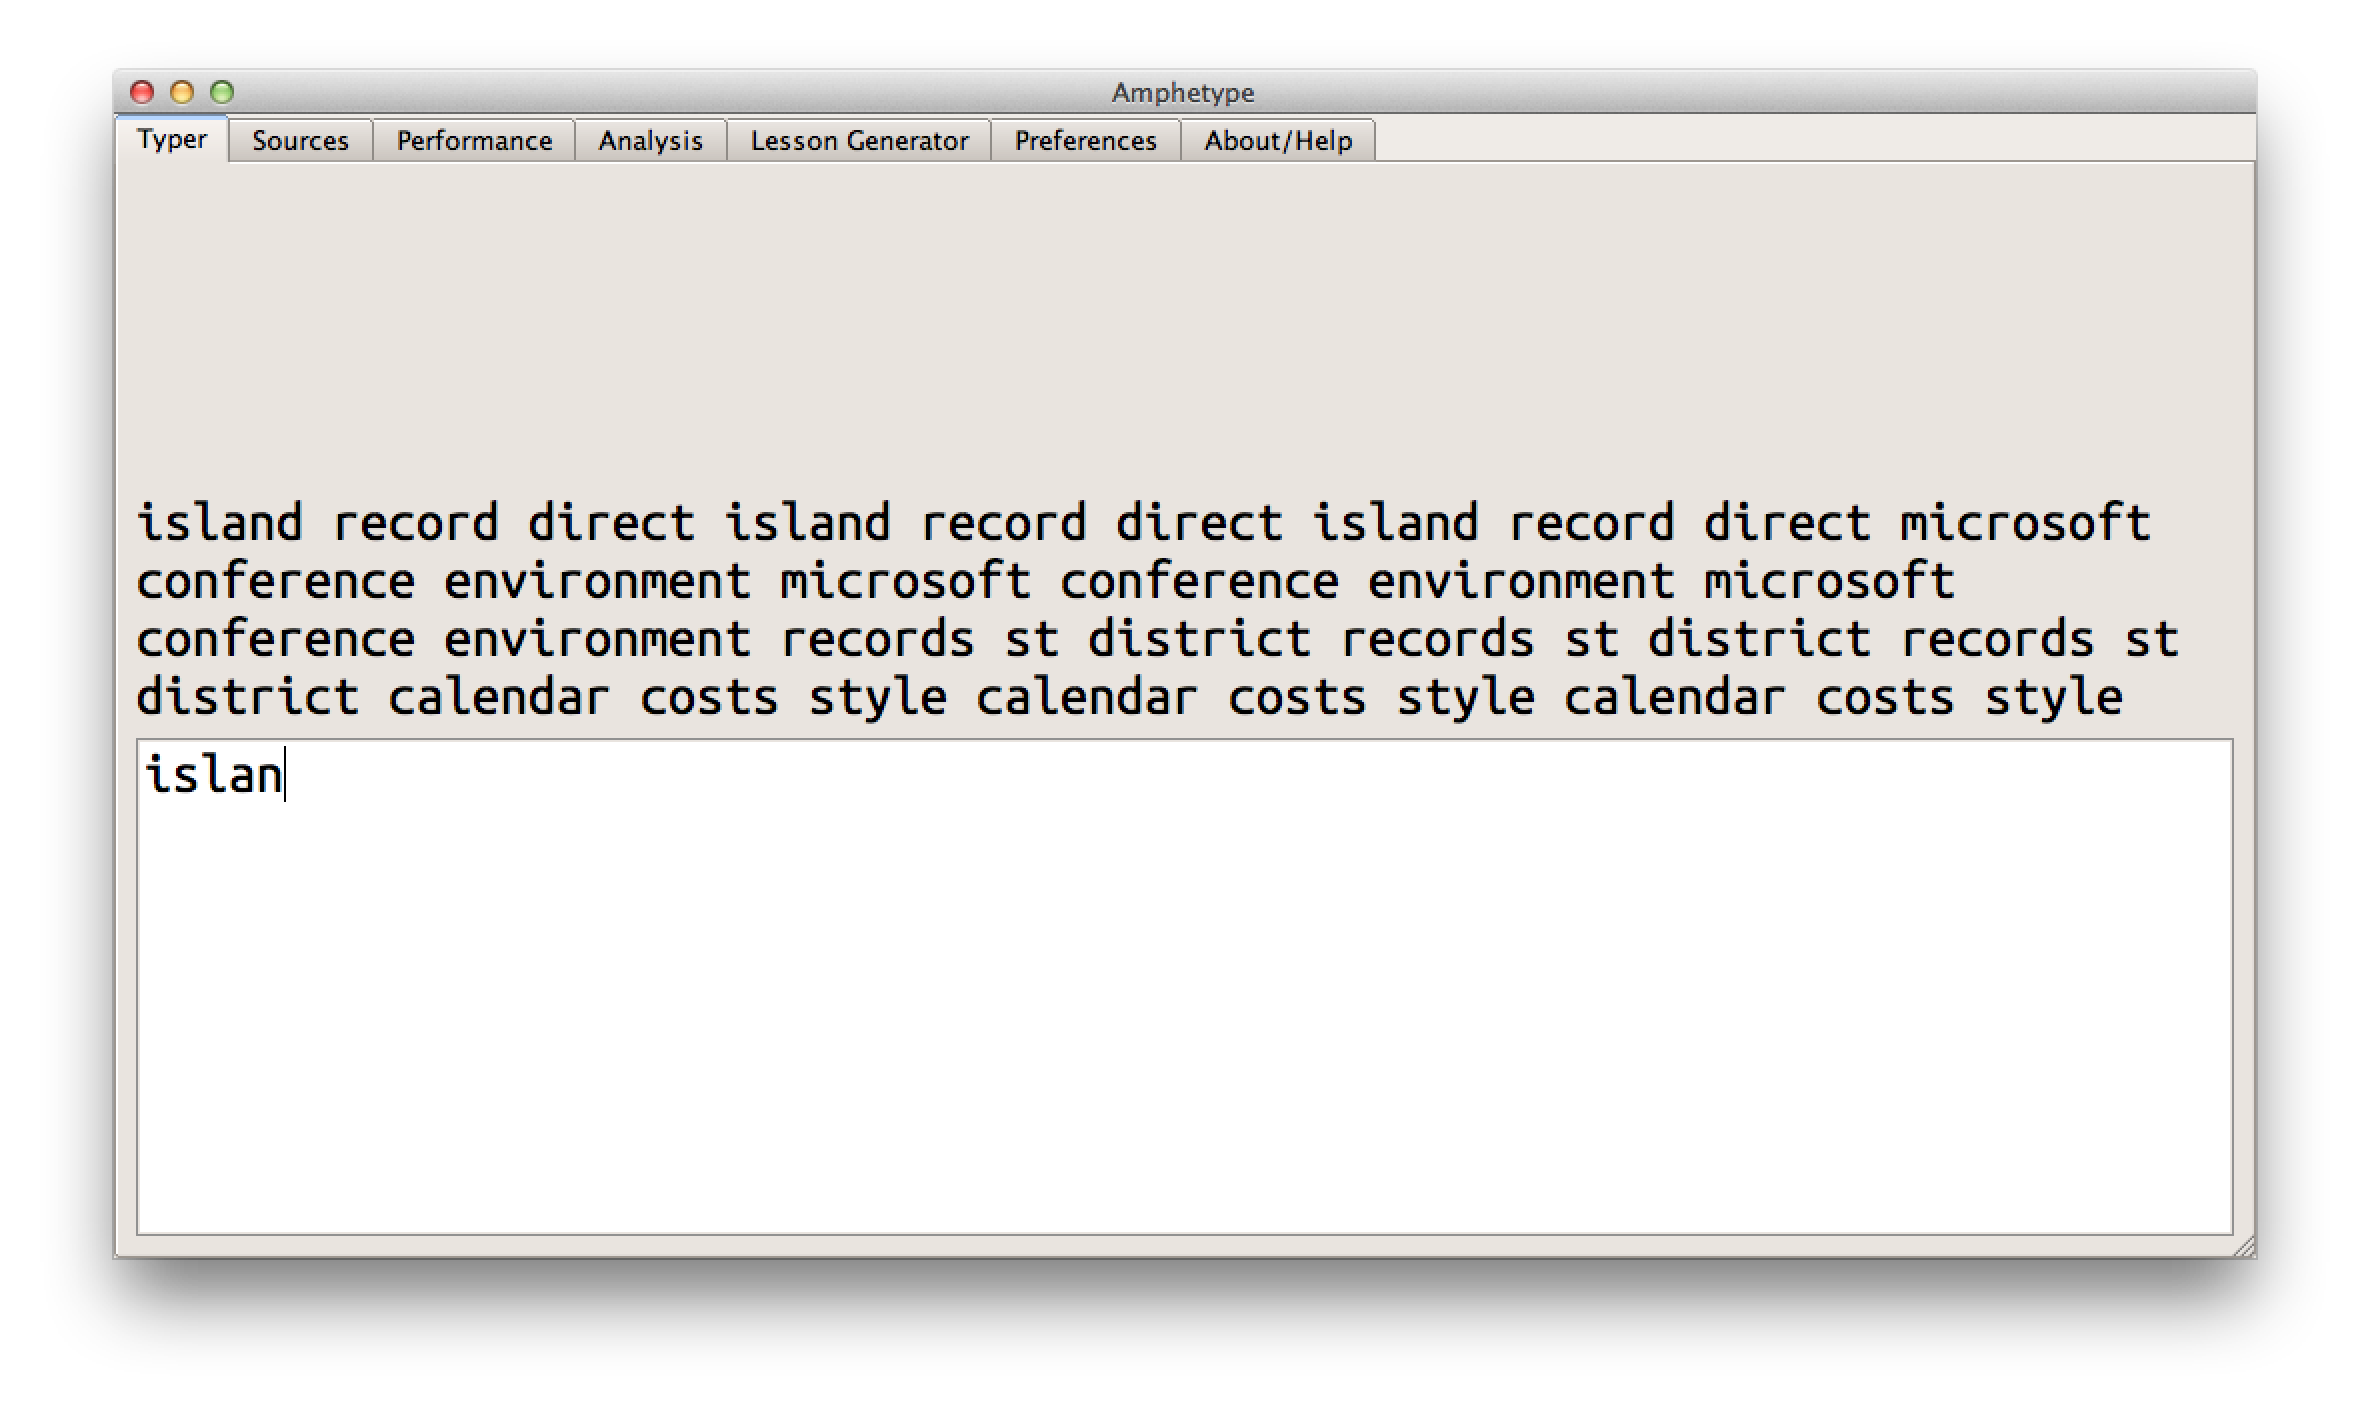
\includegraphics[width=0.8\textwidth]{amphetype-screenshot}

    \begin{itemize}
        \item Free \& open source - \url{https://code.google.com/p/amphetype/}
    \end{itemize}

\end{slide}


\begin{slide}

    \textcolor{blue}{\Large{Type-Fu}}

    \centering

    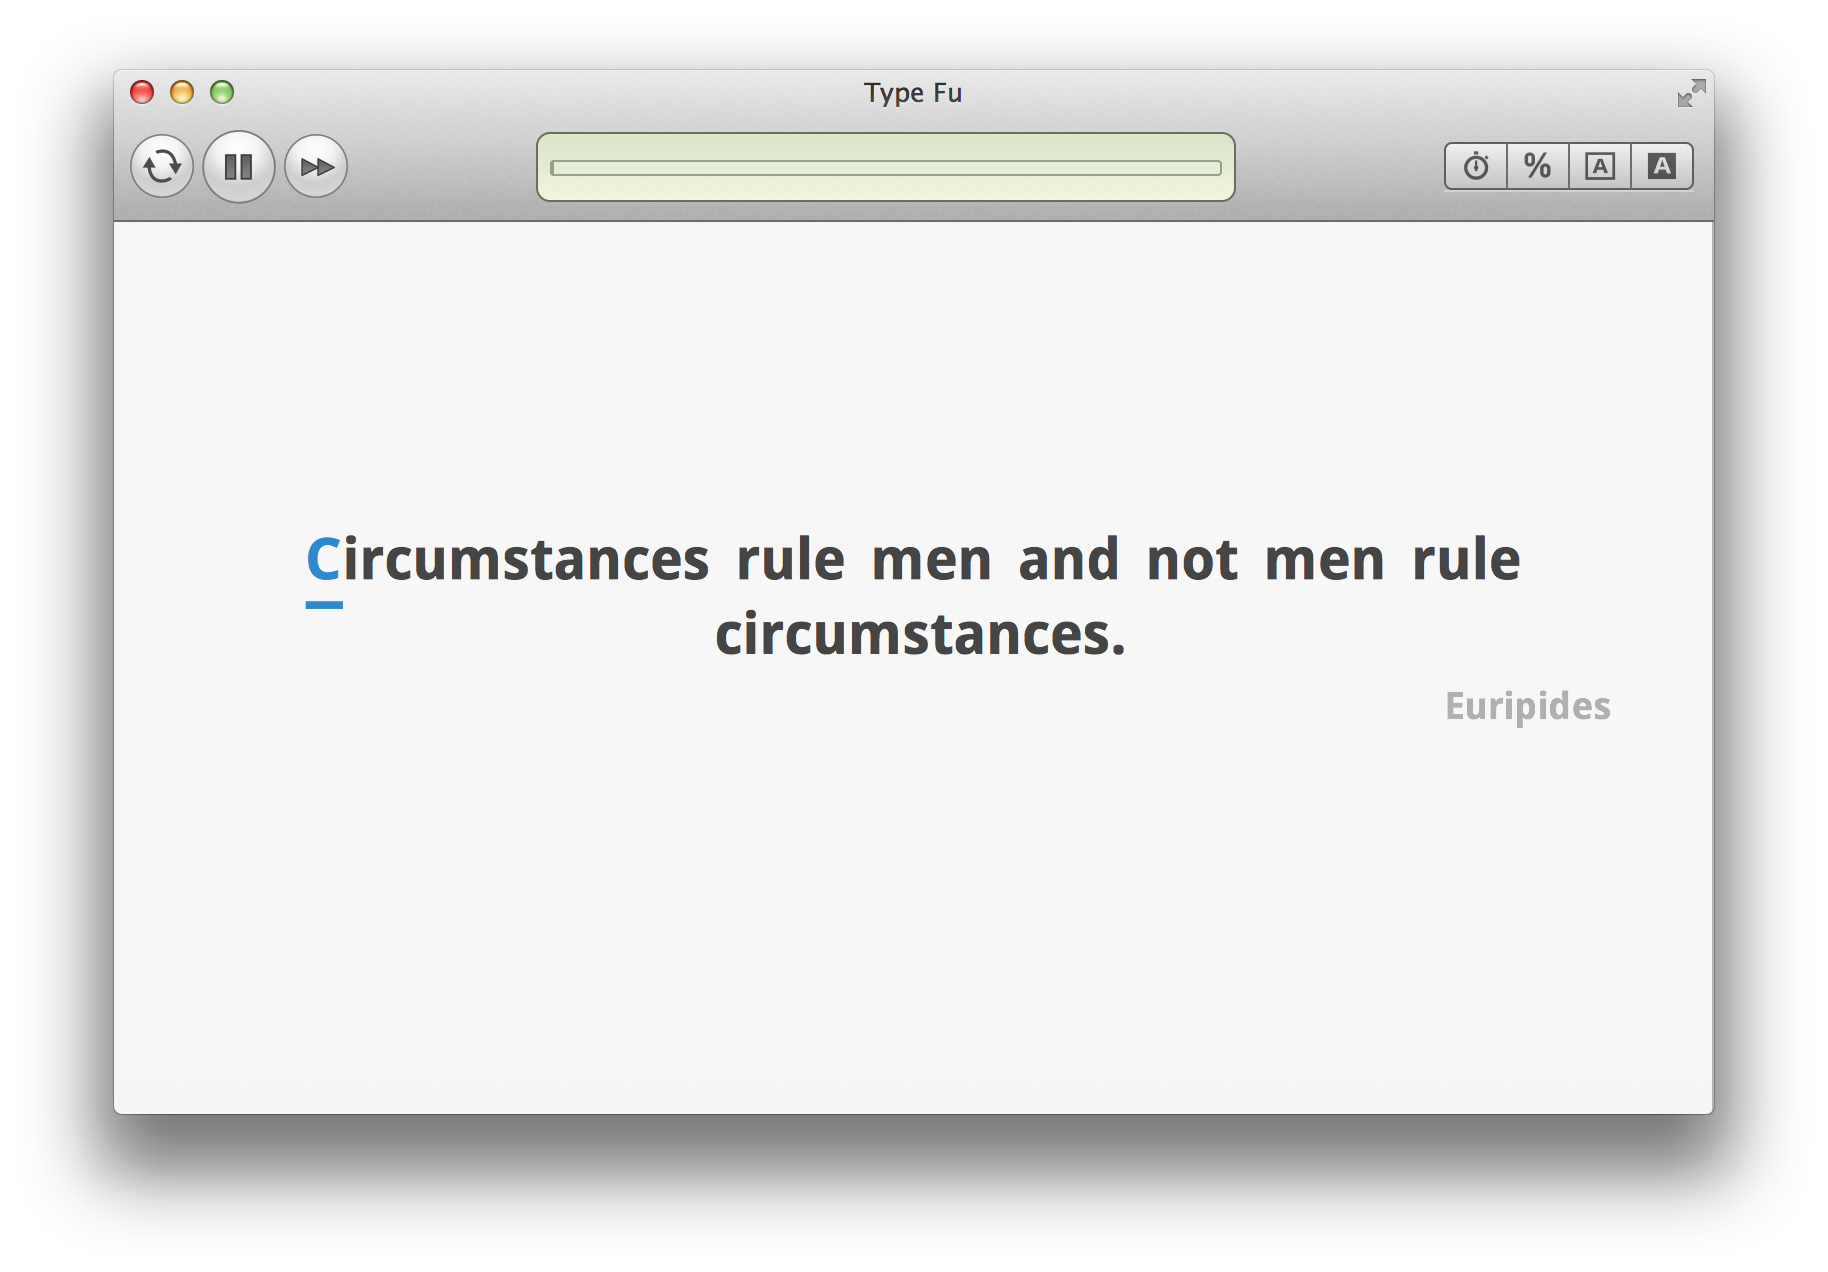
\includegraphics[width=0.8\textwidth]{type-fu-screenshot}

    \begin{itemize}
        \item $\pounds6.99$ - \url{http://type-fu.com/}
    \end{itemize}

\end{slide}


\begin{slide}

    \textcolor{blue}{\Large{Typocalypse 3D}}

    \centering

    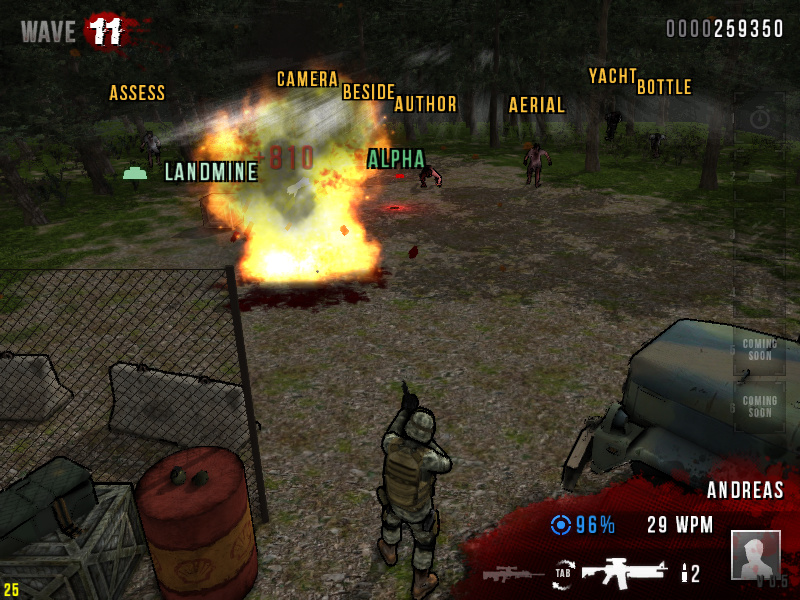
\includegraphics[width=0.75\textwidth]{typocalypse-3d}

    \begin{itemize}
        \item Free - \url{http://is.gd/typeocalypse}
    \end{itemize}

\end{slide}


\begin{slide}

    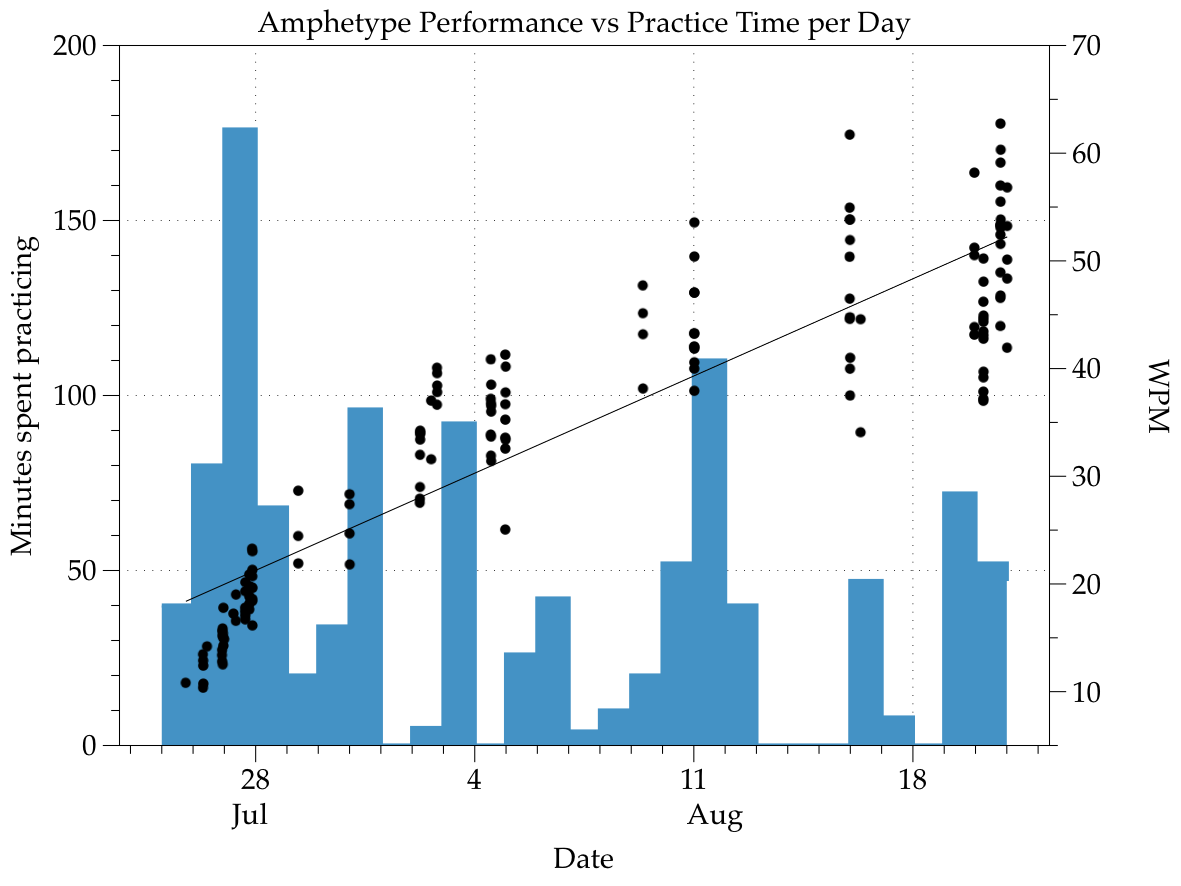
\includegraphics[width=\textwidth]{amphetype}

\end{slide}


\begin{slide}

    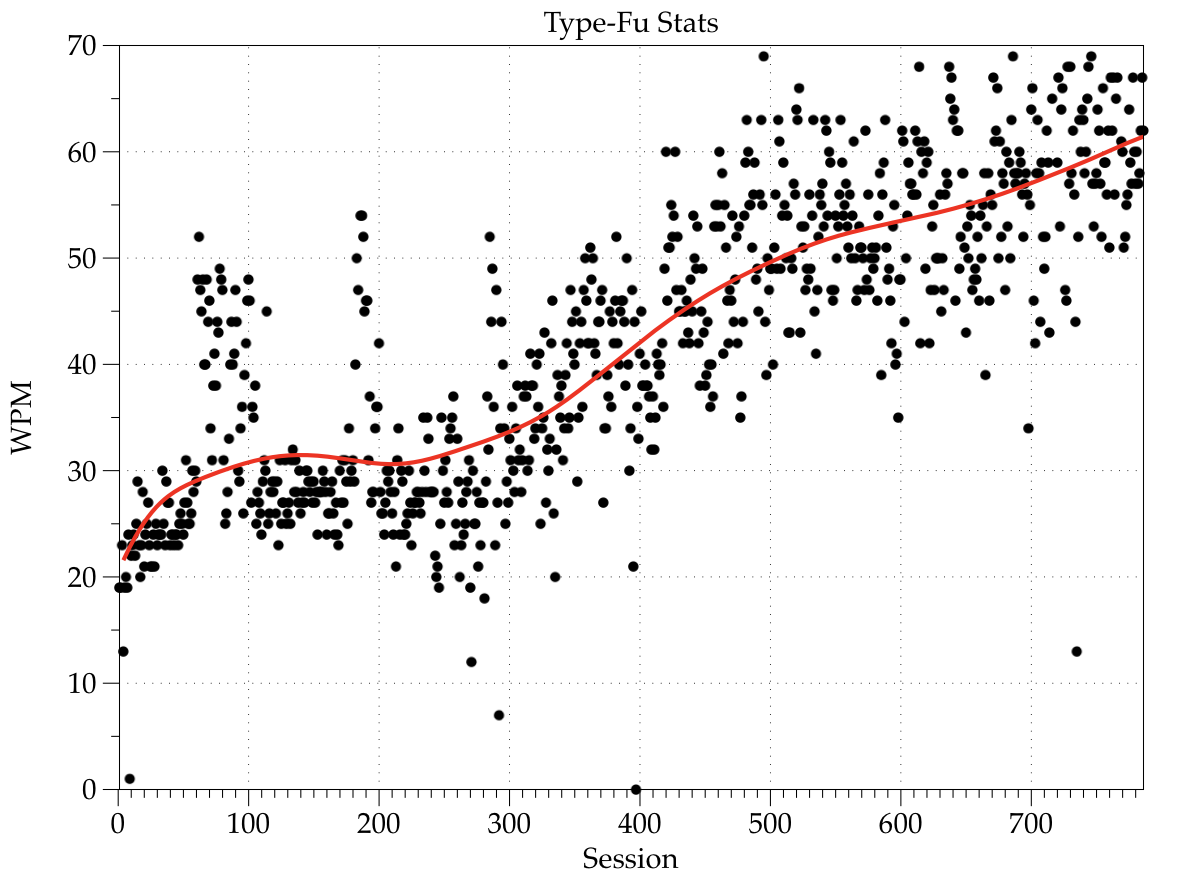
\includegraphics[width=\textwidth]{type-fu}

\end{slide}


\begin{slide}

    \textcolor{blue}{\Large{Final Statistics}}

    \begin{itemize}
        \item Total time spent practicing typing: \textbf{20:06}
        \item Moving Average WPM in Amphetype: \textbf{52 WPM}
        \item Time spent preparing this talk: \textbf{3:54}
    \end{itemize}

\end{slide}


\begin{slide}
    \textcolor{blue}{\Large{Thank you}}

    \begin{itemize}
        \item Slides on GitHub - \url{http://is.gd/adamIsDaBomb}
        \item Email me - \url{me@adamj.eu}
    \end{itemize}

\end{slide}


\end{document}
